Community detection is the problem of identifying cohesive groups of vertices, also known as clusters, in complex networks that minimize cuts and maximize internal density \cite{garza2019community}. This NP-hard problem finds applications in various domains, including drug discovery, protein annotation, topic exploration, anomaly detection, and criminal identification. Communities identified are intrinsic when based on network topology alone, and are disjoint when each vertex belongs to only one community \cite{com-gregory10}.\ignore{One of the difficulties in the community detection problem is the lack of apriori knowledge on the number and size distribution of communities \cite{com-blondel08}.} The \textit{Label Propagation Algorithm (LPA)}, also known as RAK, \cite{com-blondel08} is a popular heuristic-based approach for community detection, with the modularity metric \cite{com-newman06} being used to measure the quality of communities identified.

In the past few years, there has been an unprecedented surge in the gathering of data and the depiction of their interconnections through graphs. This surge has underscored the need for devising efficient parallel algorithms tailored for identifying communities within massive networks. The significance of the multicore/shared memory environment in this context is paramount, owing to its energy-efficient nature and the prevalence of hardware equipped with substantial DRAM capacities.\ignore{Optimizing parallel community detection algorithms for modern hardware architectures can yield notable performance benefits and competitive advantages across applications. However, many of the current algorithms for community detection are challenging to parallelize due to their irregular and inherently sequential nature \cite{com-halappanavar17}, in addition to the complexities of handling concurrency, optimizing data access, reducing contention, minimizing load imbalance.} Existing studies on LPA propose algorithmic optimizations and parallelization techniques, but do not study efficient data structures for picking the most weighted label, to the best of our knowledge. Moreover, the proposed techniques are scattered over a number of papers\ignore{, making it difficult for a reader to get a grip over them}.




\subsection{Our Contributions}

This report introduces GVE-LPA\footnote{https://github.com/puzzlef/rak-communities-openmp}, an optimized parallel implementation of LPA for shared memory multicores. On a machine with two 16-core Intel Xeon Gold 6226R processors, GVE-LPA outperforms FLPA, igraph LPA, and NetworKit LPA by $139\times$, $97,000\times$, and $40\times$ respectively. GVE-LPA is on average $5.4\times$ faster than GVE-Louvain, and achieves a processing rate of $1.4 B$ edges/s on a $3.8 B$ edge graph. With doubling of threads, GVE-LPA exhibits an average performance scaling of $1.7\times$.




%% - Use --- for a dash.
%% - Use ``camera-ready'' for quotes.
%% - Use {\itshape very} or \textit{very} for italicized text.
%% - Use \verb|acmart| or {\verb|acmart|} for mono-spaced text.
%% - Use \url{https://capitalizemytitle.com/} for URLs.
%% - Use {\bfseries Do not modify this document.} for important boldface details.
%% - Use \ref{fig:name} for referencing.

%% For a block of pre-formatted text: 
% \begin{verbatim}
%   \renewcommand{\shortauthors}{McCartney, et al.}
% \end{verbatim}

%% For a list of items:
% \begin{itemize}
% \item the ``ACM Reference Format'' text on the first page.
% \item the ``rights management'' text on the first page.
% \item the conference information in the page header(s).
% \end{itemize}

%% For a table:
% \begin{table}
%   \caption{Frequency of Special Characters}
%   \label{tab:freq}
%   \begin{tabular}{ccl}
%     \toprule
%     Non-English or Math&Frequency&Comments\\
%     \midrule
%     \O & 1 in 1,000& For Swedish names\\
%     $\pi$ & 1 in 5& Common in math\\
%     \$ & 4 in 5 & Used in business\\
%     $\Psi^2_1$ & 1 in 40,000& Unexplained usage\\
%   \bottomrule
% \end{tabular}
% \end{table}

%% For a full-width table:
% \begin{table*}
%   \caption{Some Typical Commands}
%   \label{tab:commands}
%   \begin{tabular}{ccl}
%     \toprule
%     Command &A Number & Comments\\
%     \midrule
%     \texttt{{\char'134}author} & 100& Author \\
%     \texttt{{\char'134}table}& 300 & For tables\\
%     \texttt{{\char'134}table*}& 400& For wider tables\\
%     \bottomrule
%   \end{tabular}
% \end{table*}


%% For inline math:
% \begin{math}
%   \lim_{n\rightarrow \infty}x=0
% \end{math},

%% For a numbered equation:
% \begin{equation}
%   \lim_{n\rightarrow \infty}x=0
% \end{equation}

%% For an unnumbered equation:
% \begin{displaymath}
%   \sum_{i=0}^{\infty} x + 1
% \end{displaymath}

%% For a figure:
% \begin{figure}[h]
%   \centering
%   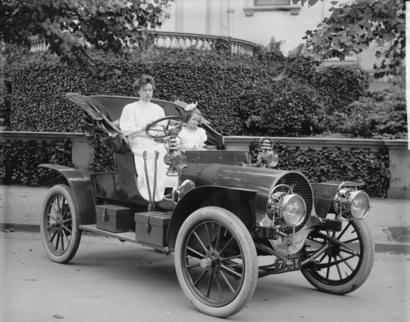
\includegraphics[width=\linewidth]{inc/sample-franklin}
%   \caption{1907 Franklin Model D roadster. Photograph by Harris \&
%     Ewing, Inc. [Public domain], via Wikimedia
%     Commons. (\url{https://goo.gl/VLCRBB}).}
%   \Description{A woman and a girl in white dresses sit in an open car.}
% \end{figure}

%% For a teaser figure.
% \begin{teaserfigure}
%   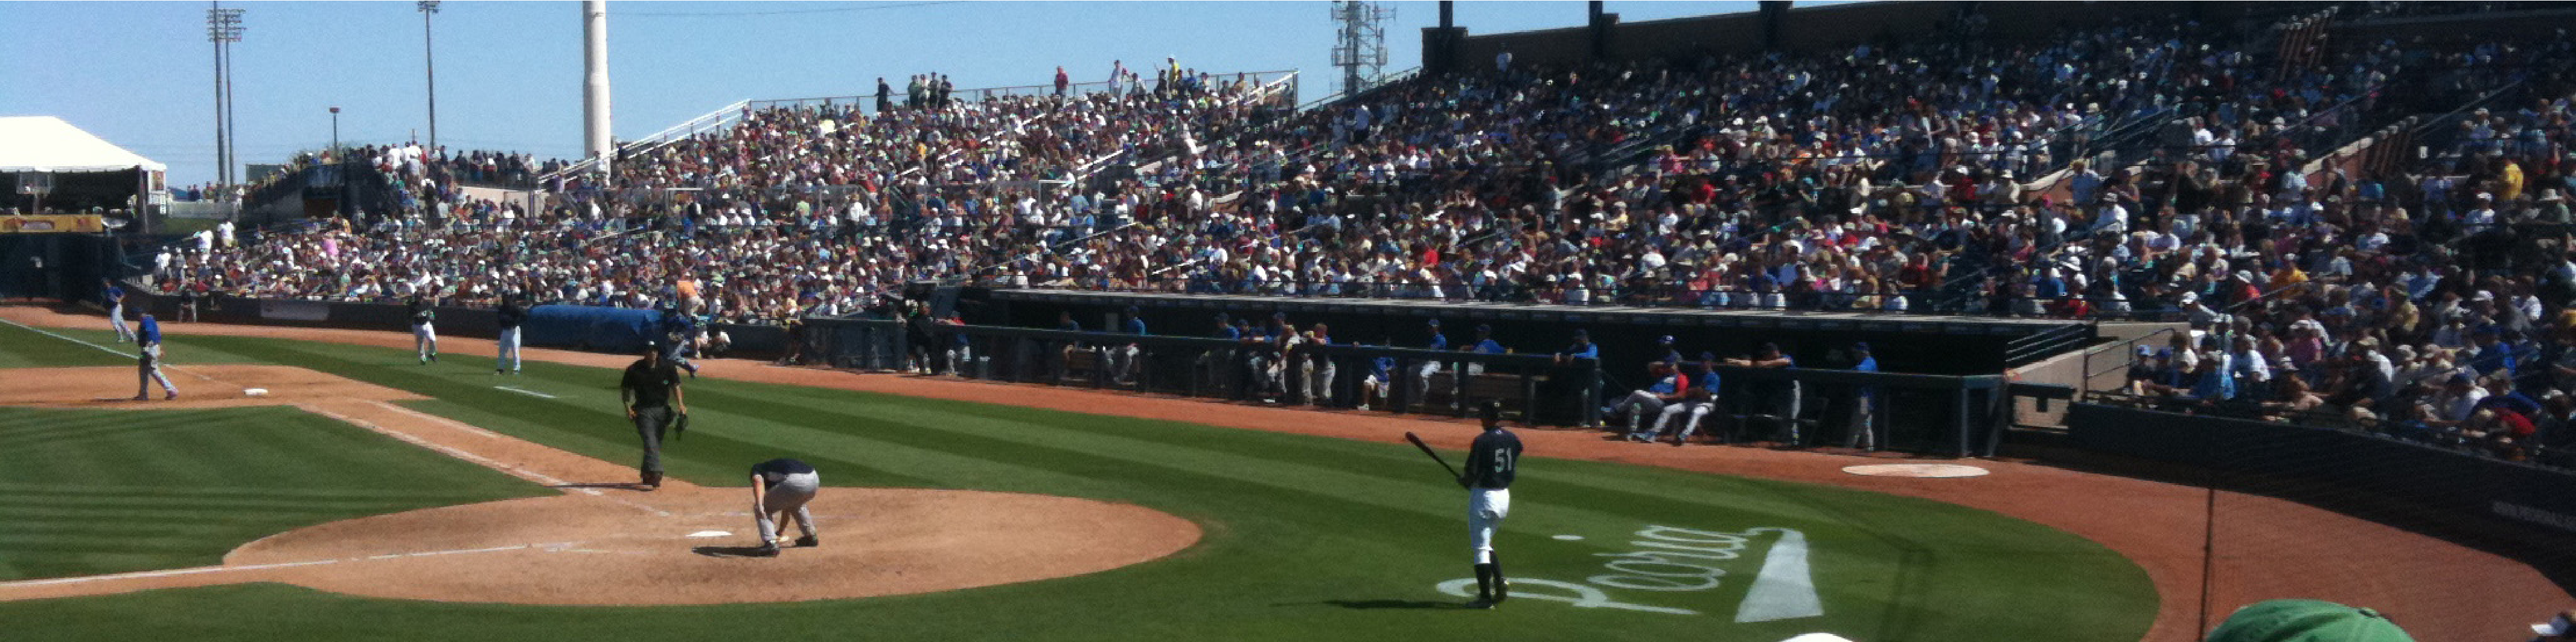
\includegraphics[width=\textwidth]{sampleteaser}
%   \caption{figure caption}
%   \Description{figure description}
% \end{teaserfigure}
